\chapter{Analyse eines Entwicklungssystems}\label{chap:analyse}
\minitoc
In diesem Kapitel soll aufgezeigt werden, woraus ein Entwicklungssystem
im Allgemeinen besteht und welche Anforderungen sich also für ein zu
entwerfendes Entwicklungssystem ergeben.
\section{Begriffsdefinitionen}
\subsection*{Zielsystem}
Das \emph{Zielsystem} ist das zu entwerfende Entwicklungsziel.
\subsection*{Entwicklungsplattform}
Zu einer \emph{Entwicklungsplattform} gehören alle Hardware- und
Softwareelemente, die nötig sind, um die Umsetzung eines bestimmten
Softwareprojektes zu erreichen. Die einzelnen Bestandteile einer solchen
\emph{Entwicklungsplattform} sollen im Verlauf dieses Kapitels identifiziert
werden.
\section{Elemente einer Entwicklungsplattform}
Die Elemente einer Entwicklungsplattform lassen sich grob drei Kategorien
zuordnen. 

Viele Teile dieser drei Kategorien beeinflussen Entscheidungen, die für
einen anderen Bereich getroffen werden müssen.
\subsection{Vorgehensmodell}
Zu jedem Entwicklungsprozesses gehört auch immer die Entscheidung über eine
Vorgehensweise. Viele Vorgehensweisen basieren dabei auf Vorgehensmodellen,
die in Industrie und Wirtschaft weit verbreitet sind. Als Beispiele lassen sich
hier das Wasserfallmodell, das V-Modell, Scrum oder auch Extreme Programming
nennen.

All diesen Modellen ist gemein, dass einige ihrer Schritte
unbedingt Unterstützung durch Soft- und Hardware bedürfen oder
diese die Entwicklung unter Umständen beschleunigen kann.

Da es eine klare Strukturierung zeigt, soll hier exemplarisch für alle
Vorgehensmodelle das \textbf{Wasserfallmodell} aufgeführt werden.

Andere Vorgehensmodelle strukturieren ihren Ablauf unterschiedlich, jedoch sind
diese Unterschiede für die Wahl der verwendeten Hard- und Software nur von
untergeordneter Relevanz, da die zentralen Entwicklungsschritte
identisch sind.

\subsubsection*{Wasserfallmodell}
Das Wasserfallmodell ist ein klassisches, nicht-iteratives Vorgehensmodell,
dessen Ablauf man sich anhand eines Wasserfalls gut visualisieren kann. 

\begin{figure}[!h]
\centering
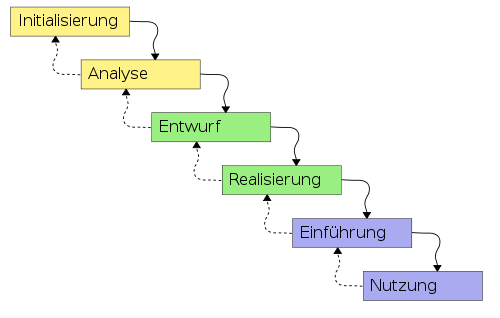
\includegraphics[width=350pt]{wasserfallmodell.png}
\caption{Ablauf eines Softwareprojektes nach dem Wasserfallmodell Aufgenommen:
12.03.2013}
\end{figure}

Jeder einzelne Schritt in der Entwicklung stellt hierbei eine abgeschlossene
Phase mit vorher festgelegten Anfangs- und Endpunkten dar.

In den Initialisierungs- und Analysephasen wird oft der Kunde in die
Entwicklung eingebunden. Typischerweise werden hier deshalb keine oder nur
wenige spezialisierte Tools verwendet. Zu der verwendeten Software zählt hier
unter anderem \emph{Projektmanagementsoftware}.

Die Entwurfs- und Realisierungsphasen jedoch benötigen oft eine hohe
Softwareunterstützung. Während in der Entwurfsphase meist Tools zur
Visualisierung und Strukturierung von Softwarearchitektur eingesetzt werden
\emph{(UML, Struktogramme, etc.)}, werden in der Realisierungsphase meist
Werkzeuge eingesetzt, die von der konkreten Anforderung abhängen.
\emph{(Compiler, IDEs, Debugger)}

Um einen Übergang in die Einführungs- und Nutzungsphasen zu ermöglichen, muss
die Software beziehungsweise das Gesamtsystem oft Tests durchlaufen, die das
System auf eine Erfüllung der Anforderungen überprüfen. Hierfür werden
Testpraktiken benutzt, die auch oft auf Soft- und Hardwaregestützt ablaufen.
\emph{(JTAG, Unittests, In-circuit Tests)}

Auch durchläuft ein System in seiner Nutzungsphase oft auch Wartungszyklen.
Diese Zyklen setzen eine möglichst einfache Wartbarkeit des Systems voraus.

\subsection{Software}\label{sub:software}
Software unterstützt Softwareprojekte in allen Phasen der Durchführung.

Obwohl viele dieser einzelnen Elemente auf Hardwareunterstützung angewiesen
sind, sollen in diesem Abschnitt nur die Softwarebestandteile beschrieben
werden. Soweit es nötig ist, werden die zugehörigen Gegenstücke in
\autoref{sub:hardware} beschrieben.
\begin{itemize}
  \item \subsubsection*{IDEs} IDEs\footnote{Integrated Development Environment}
  sind zentrale Entwicklungsoberflächen der Softwareentwickler. In dieser
  Umgebung werden oftmals viele Tools zusammengefasst, die für den
  Entwicklungszyklus notwendig sind. Sie dienen dazu Quelltext zu verwalten und
  zu schreiben, Versionsverwaltung zu betreiben, Code zu kompilieren, die
  entwickelte Software zu testen, zu deployen und zu debuggen.
  
  Oft werden die in den folgenden Punkten aufgeführten Tools in eine IDE
  integriert, um Entwicklungsabläufe zu vereinfachen und zu beschleunigen.
  
  \emph{Beispiele:} Eclipse, NetBeans, CodeWarrior, Microsoft Visual Studio, Qt
  Creator
  \item \subsubsection*{Compiler} Compiler sind für viele Softwareprojekte von
  essentieller Bedeutung. Speziell im eingebetteten Bereich werden überwiegend
  kompilierte Programmiersprachen wie C oder C++ eingesetzt, da sie nach dem
  Kompiliervorgang in nativem Maschinencode vorliegen und so oft eine höhere
  Ausführungsgeschwindigkeit gewährleisten können. Außerdem können sie meist
  besser an das Zielsystem angepasst werden, da sie keiner weiteren Frameworks
  oder Interpreter mit "`überflüssigen"' Funktionen bedürfen.
  
  Soll eine kompilierte Software auf einem anderen als dem Entwicklungssystem
  eingesetzt werden, so wird ein sogenannter \textbf{Cross-Compiler} benötigt.
  Diese speziellen Compiler sind in der Lage, Software zu kompilieren, die
  später auf einer andere Rechnerarchitektur (z.B. ARM statt Intel) und/oder auf
  einem anderen Betriebssystem (z.B. Linux statt Windows) betrieben werden soll.
  
  \emph{Beispiele:} GCC, IAR C/C++ Compiler, ARM RVCT Compiler, Intel C++
  Compiler, CodeWarrior Compiler
  \item \subsubsection*{Debugger}\label{subs:swdebugger} Der Debugger ist ein
  Tool, mithilfe dessen ein Entwickler eine Software während ihrer Laufzeit
  untersuchen, steuern und, in einem gewissen Rahmen, modifizieren kann. Er
  dient dem Entwickler hauptsächlich zur Fehlersuche, da es mit seiner Hilfe
  sehr leicht ist, die Vorgänge in einer Software nachzuvollziehen.
  
  Der Entwickler ist durch das Setzen von Breakpoints\footnote{Willkürliche,
  vom Entwickler vor dem Start der Software zu setzende, "`Haltepunkte"' im
  Programmablauf.} mittels des Debuggers in der Lage, eine Software in einen
  definierten Zustand zu bringen. Anschließend kann er den weiteren
  Programmablauf schrittweise ausführen lassen (single-stepping) oder mitunter
  auch geringfügige Änderung am Speicher des Systems vornehmen.
  
  Debugger sind in integrierten Systemen oft auf eine hohe Hardwareunterstützung
  angewiesen. In \autoref{subs:hwdebugger} wird dies näher beschrieben.
  
   \emph{Beispiele:} GDB (GNU Debugger), IDB (Intel Debugger), Valgrind
  \item \subsubsection*{Testtools} In die Kategorie der Testtools fallen
  alle Elemente die benötigt werden, um die Funktionsfähigkeit eines Systems zu
  prüfen. Außerdem dienen diese auch oft dazu, ein Gesamtsystem sowie dessen
  Teilsysteme auf die Erfüllung der Anforderungen zu prüfen.
  
  Um die einzelnen Bestandteile eines Systems zu überprüfen, existieren viele
  verschiedene Ansätze. Meist werden Tests grob in \emph{Modultests},
  \emph{Integrationstests}, \emph{Systemtests} und \emph{Abnahmetests}
  unterteilt.
  
  Alle diese Testarten setzen jedoch eine grundlegende Testbarkeit des Systems
  voraus.
  
  \emph{Beispiele:} Unittests, \ldots  
  \item \subsubsection*{Deploymenttools}\label{subs:deployment} Um ein System
  ausliefern zu können, muss es für den Endanwender vorbereitet werden.
  
  Im Embeddedbereich erfolgt dies meist durch ein "`Flashen"' der Firmware.
  Dieser Vorgang wird jedoch, zu Testzwecken, auch in der Entwicklungsphase
  eines Projektes oft durchgeführt und muss daher entsprechend einfach und
  möglichst unkompliziert sein.
  
  \emph{Beispiele:} Installer, Paketverwaltungssysteme, Skripte
\end{itemize}

\subsection{Hardware}\label{sub:hardware}
Die für ein Projekt benötigte Hardware wird oftmals\ldots
\begin{itemize}
  \item \subsubsection*{Testtools} Um Tests durchführen zu können, wird
  oft auch eine Unterstützung durch Hardware benötigt. Der JTAG\footnote{Joint
  Test Action Group}-Port bietet hier oftmals eine der zentralen
  Möglichkeiten, das System zu testen.
  \item \subsubsection*{Debugger}\label{subs:hwdebugger}  Um
  Softwaredebugging wie in \autoref{subs:swdebugger} beschrieben im Umfeld eines
  Mikroprozessors zu erleichtern beziehungsweise überhaupt zu ermöglichen,
  besitzen diese oft verschiedene Eigenschaften.
  Um eine Software Schritt-für-Schritt auszuführen, wird eine Unterstützung von
  der CPU vorausgesetzt. Prozessorkerne der ARM-Architektur lassen sich zum
  Beispiel über einen sogenannten TAP\footnote{test access
  port} oder DAP\footnote{Debug Access Port; benutzt von neueren ARM Kernen.
  Ermöglicht Tracing} in einen Debug-Modus bringen.
  Dieser Debug-Modus ist Voraussetzung dafür, Single-Step-Debugging duchführen
  oder Breakpoints setzen zu können.
  
  Der JTAG-Port stellt oft die Schnittstelle
  zu diesen Modulen dar.
  
  Neben einer JTAG-Schnittstelle und der Möglichkeit, ein System mittels
  In-System Programmer\footnote{Anschluss der es erlaubt, ein integriertes
  System wie einen Mikrocontroller mit einer Software zu programmieren, ohne
  ihn ausbauen zu müssen.} programmieren zu können, erlauben es zum Beispiel
  viele Mikroprozessoren, Breakpoints im Programm zu setzen.
  \item \subsubsection*{Flasher} Um, wie in \autoref{subs:deployment}
  beschrieben, ein Zielsystem mit einer Firmware beschreiben zu können, wird oft
  ein Hardwarebaustein benötigt.
  
  Abhängig vom verwendeten Zielsystem erfolgt ein "`Flashen"' meist über extra
  dafür bestimmte Hardware. Gängige Varianten sind hierbei zum Beispiel das
  ISP\footnote{In-system programming} sowie die Verwendung des JTAG-Ports zur
  Übertragung des Programmcodes.
\end{itemize}
\section{Vorgaben} In diesem Abschnitt sollen die Vorgaben für ein
beispielhaftes Zielsystem festgelegt werden. 

Das zu entwerfende Entwicklungssystem soll dabei ein möglichst großes Spektrum
potentieler Architekturen und Funksysteme abdecken können, so dass es später
einfach ist, das zu entwickelnde Zielsystem durch ein anderes zu ersetzen.
\subsection{Analyse/Marktübersicht}
\subsubsection{Prozessorarchitekturen} => Wir wollen ARM
\subsubsection{Funkmodule} => Wir wollen einen Transceiver ohne übermäßige
interne Logik
\subsection{Festlegung} In diesem Abschnitt soll festgelegt
\subsubsection{ARM als Zielplattform} => Warum der ARM von Olimex gut ist
\subsubsection{MRF24J40 als Funkmodul} => Warum dieses Modul die einfachste Wahl
ist
\section{Anforderungen an ein konkretes System (Lastenheft)}
\subsection{Debugging} Warum wir OpenOCD/GDB brauchen
\subsection{Deployment} Warum wir JTAG zum Flashen brauchen
\subsection{Datenanalyse} Warum wir UART Output brauchen





\iffalse

%%=============================================================================
\section{Softwareunterstützung}
Für eine neue Entwicklungsplattform ist es wünschenswert, sich nicht von einem
speziellen Vorgehensmodell abhängig zu machen. Es sollte also eine Schnittmenge
gefunden werden, um die Minimalanforderungen möglichst vieler Modelle abdecken
zu können.

Als Schnittmenge kristallisieren sich dabei folgende Aspekte heraus:
\begin{itemize}
  \item \subsection*{Programmieren} Eine Softwareunterstützung erfolgt in diesem
  Schritt meist durch eine IDE und/oder einen Compiler.
  \item \subsection*{Testen} Je nach Art der Tests wird auch in diesem Schritt
  Softwareunterstützung benötigt. 
  \item \subsection*{Verteilen} Soll eine Software auf mehrere
  Systeme verteilt werden, passiert dies fast immer softwaregestützt.
  \item \subsection*{Warten} Die Wartung einer Software ist ein weiterer
  wichtiger Bestandteil des Softwarelebenszyklus'.
\end{itemize}
\section{Vorbedingungen durch das zu entwickelnde System}\label{sec:vorb}
Entwicklung von Software für funkende Mikrocontroller. Dies Mikrocontroller sind
teilweise hochgradig in ihre Umgebung integriert. So können diese z.B.
nicht für die Entwicklung kurzfristig ausgebaut werden. Aufgrund ihrer extrem
hohen Verbreitung\footnote{Referenz} bezieht sich diese Arbeit ausschließlich
auf Systeme mit ARM-Architektur.
\section{Weitere Gegebenheiten}\label{sec:gegeb}
Es existiert Infrastruktur, die man sich für die Entwicklung zu Nutze machen
kann. Hierzu zählen zum Beispiel WLAN, Stromversorgung, Ethernet.

\section{Randbedingungen des Entwicklungsprozesses}
Die gegebenen Umständen aus \autoref{sec:gegeb} und \autoref{sec:vorb} ergeben
folgende Randbedingungen:
\begin{itemize}
  \item Das Zielsystem ist nie auch gleichzeitig das Entwicklungssystem.
  Zusätzlich zu der Tatsache, dass die Zielsysteme eine andere
  \item Das Zielsystem interagiert mit Umgebung. Deshalb sind zum Beispiel
  Funkstörungen o.Ä. zu beachten
  \item Der Zielsystemort ist selten auch der Entwicklungsort
  \item Es existieren viele Zielsysteme mit gleicher oder ähnlicher
  Konfiguration
\end{itemize}

\section{Anforderungen an das Entwicklungssystem}
Aus den Randbedingungen ergeben sich harte und weiche Anforderungen an ein
potentielles Entwicklungssystem. Die harten Anforderungen müssen von einem
Entwicklungssytem zwangsweise erfüllt werden um als geeignetes System dienen zu
können. Die Erfüllung weicher Anforderungen kann den den
Entwicklungsprozess vereinfachen und dem Entwickler die Arbeit erleichtern.
\subsection{Harte Anforderungen}
\begin{itemize}
  \item Schon während der Entwicklung muss ein Zugriff auf das Zielsystem zum
  Debuggen möglich sein
  \item Software muss "`remote"' deployt werden können
  \item Tests sollten aus Simulationsgründen vor Ort erfolgen
  \item Wartungszyklen und Wartungsupdates müssen meist für viele Systeme
  parallel duchgeführt werden
\end{itemize}
\subsection{Weiche Anforderungen}
\begin{itemize}
  \item 
\end{itemize}


\section{Entwicklungsmodelle}
Unterschiedliche Anforderungen je nach Entwicklungsziel
Manche stimmen jedoch überein, so z.B.
  



Abhängig von den Vorfaben und den eingesetzten Entwicklungsmodellen werden
für jedes Softwareprojekt unterschiedliche Anforderungen an die verwendete Hard-
und Software gestellt.

Diese Anforderungen 

 Je nach Art der Software, Anforderungen und

Unabhängig von der Wahl des Entwicklungsmodells können und
müssen viele dieser Schritte teilweise auch softwaregestützt ablaufen. Es ist
daher für ein Entwicklungssystem zwingend notwendig, diese Schritte zu
unterstützten.

Zu den softwaregestützten Schritten zählen hierbei:
\begin{itemize}
  \item \subsection*{Modultest} Modultest
  \item \subsection*{Integrationstest} Integrationstest eingebetteter Systeme
  erfolgen meist mit Hilfe standardisierter Verfahren. Diese verfahren lassen
  sich oft auch zum Beispiel in die Endkontrolle von herstellungsprozessen
  integrieren. So sind in der Industrie verfahren wie JTAG oder Pintests weit
  verbreitet.
  \item \subsection*{Deployment} Im Bereich der 
  \item \subsection*{Wartung}
\end{itemize}

\ldots
\section{JTAG}
JTAG statt SWD
\begin{itemize}
  \item Wird von viele Prozessoren unterstützt.
  \item Ermöglicht ein umfangreiches Debuggen des Prozessors bis auf
		Registerebene.
  \item OpenOCD hat bereits viele Funktionen.
\end{itemize}
\section{Netzwerkprotokoll}
\subsection{Zeitsynchronisation}
\section{Serversoftware}

\section{Clientsoftware}
\fi